\documentclass{article}
\usepackage{tikz}
\usetikzlibrary{automata,positioning}

\begin{document}

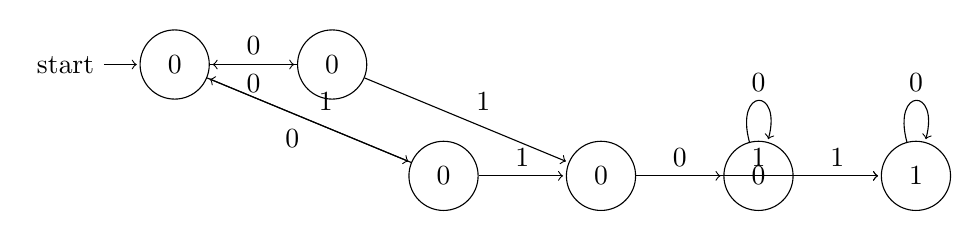
\begin{tikzpicture}[shorten >=1pt,node distance=2cm,on grid,auto]
    \node[state,initial] (q_0) {$0$};
    \node[state] (q_1) [right of=q_0] {$0$};
    \node[state] (q_2) [below right of=q_1] {$0$};
    \node[state] (q_3) [right of=q_2] {$0$};
    \node[state] (q_4) [right of=q_3] {$0$};
    \node[state] (q_5) [right of=q_4] {$1$};

    \path[->]
    (q_0) edge node {0} (q_1)
          edge node {1} (q_2)
    (q_1) edge node {0} (q_0)
          edge node {1} (q_3)
    (q_2) edge node {0} (q_0)
          edge node {1} (q_3)
    (q_3) edge node {0} (q_4)
          edge node {1} (q_5)
    (q_4) edge [loop above] node {0} ()
          edge node {1} (q_5)
    (q_5) edge [loop above] node {0} ();
\end{tikzpicture}

\end{document}